\documentclass[11pt,a4paper]{article}

\usepackage[utf8]{inputenc}
\usepackage[T1]{fontenc}
\usepackage{lmodern}
\usepackage[margin=2.2cm]{geometry}
\usepackage{graphicx}
\usepackage{booktabs}
\usepackage{tabularx}
\usepackage{longtable}
\usepackage{array}
\usepackage{enumitem}
\usepackage[table]{xcolor}
\usepackage{listings}
\usepackage{fancyhdr}
\usepackage{titlesec}
\usepackage[hidelinks]{hyperref}

\definecolor{brand}{HTML}{1E3A8A}
\definecolor{must}{HTML}{B91C1C}
\definecolor{should}{HTML}{B45309}
\definecolor{may}{HTML}{047857}
\definecolor{codebg}{HTML}{F6F8FA}
\definecolor{rule}{HTML}{D0D7DE}

\titleformat{\section}{\Large\bfseries\color{brand}}{\thesection}{0.8em}{}
\titleformat{\subsection}{\large\bfseries\color{brand}}{\thesubsection}{0.8em}{}

\pagestyle{fancy}
\fancyhf{}
\lhead{\small City Brain Convergence -- Interface Specification}
\rhead{\small v0.1 (draft)}
\cfoot{\small\thepage}
\renewcommand{\headrulewidth}{0.4pt}

\newcommand{\code}[1]{\texttt{#1}}
\newcommand{\MUST}{\textbf{\textcolor{must}{MUST}}}
\newcommand{\SHOULD}{\textbf{\textcolor{should}{SHOULD}}}
\newcommand{\MAY}{\textbf{\textcolor{may}{MAY}}}
\newcolumntype{Y}{>{\raggedright\arraybackslash}X}

\lstset{
  basicstyle=\ttfamily\small,
  backgroundcolor=\color{codebg},
  frame=single, rulecolor=\color{rule},
  breaklines=true, columns=fullflexible,
  showstringspaces=false, xleftmargin=4pt, xrightmargin=4pt,
  aboveskip=8pt, belowskip=8pt
}

\setlist{itemsep=2pt,topsep=4pt}
\renewcommand{\arraystretch}{1.25}
\setlength{\parindent}{0pt}
\setlength{\parskip}{5pt}

\begin{document}

%-------------------------------------------------------------------
\begin{titlepage}
\centering
\vspace*{3cm}
{\Large\color{brand} TSYP14 Technical Challenge -- City Brain Convergence\par}
\vspace{1.2cm}
{\Huge\bfseries Interface Specification Book\par}
\vspace{0.6cm}
{\LARGE What the City Brain layer expects from\\ the Twin and Guardian layers\par}
\vspace{1.5cm}
{\large Version 0.1 -- draft for review by the triplet\par}
\vspace{0.3cm}
{\large 15 October 2026\par}
\vfill
\begin{tabularx}{0.85\linewidth}{@{}lY@{}}
\toprule
\textbf{Prepared by} & City Brain layer team \\
\textbf{For} & Twin layer team, Guardian layer team \\
\textbf{Status} & Proposal. Every item is open to discussion until the interface freeze. \\
\textbf{Scope} & Communication, security and message contents between the three layers \\
\bottomrule
\end{tabularx}
\vspace{1cm}
\end{titlepage}

\tableofcontents
\newpage

%-------------------------------------------------------------------
\section{Introduction}

\subsection{Purpose}
This book describes, as precisely as possible, \textbf{what the City Brain layer needs to receive} from the Twin and Guardian layers, and \textbf{what it sends back}. Its goal is that each team can build its layer, and its mocks of the other layers, independently, and that the three layers work together the first time they are connected.

It covers only what crosses the boundary between layers. How each team builds the inside of its layer is free.

\subsection{Decisions already taken}
\begin{itemize}
  \item \textbf{MQTT} is the communication protocol between all layers.
  \item \textbf{TLS} protects every connection; every message carries an \textbf{HMAC}, a \textbf{timestamp} and a \textbf{unique id}.
  \item Each layer runs on its own with \textbf{mocks} of the other two (Phase 1 requirement R1).
\end{itemize}

\subsection{How to read the requirements}
Each requirement has an identifier and a level:

\begin{tabularx}{\linewidth}{@{}lY@{}}
\toprule
\MUST & Required for the layers to work together. Without it, integration fails. \\
\SHOULD & Strongly recommended. It can be skipped only with a good reason, agreed by the triplet. \\
\MAY & Optional. Useful if time allows. \\
\bottomrule
\end{tabularx}

\medskip
Identifiers: \code{TR} transport, \code{SEC} security, \code{MSG} message format, \code{TW} Twin layer, \code{GD} Guardian layer, \code{BR} City Brain layer, \code{IT} integration tests.

\subsection{Changes to this document}
\begin{itemize}
  \item This version is a \textbf{draft}. Comments are welcome until the interface freeze date agreed by the triplet.
  \item After the freeze, any change is announced in the triplet channel, written in this document with a new version number, and reflected in the shared \code{INTEGRATION.md}.
  \item No layer changes a topic name or a message field silently.
\end{itemize}

%-------------------------------------------------------------------
\section{System overview}

\begin{figure}[h]
\centering
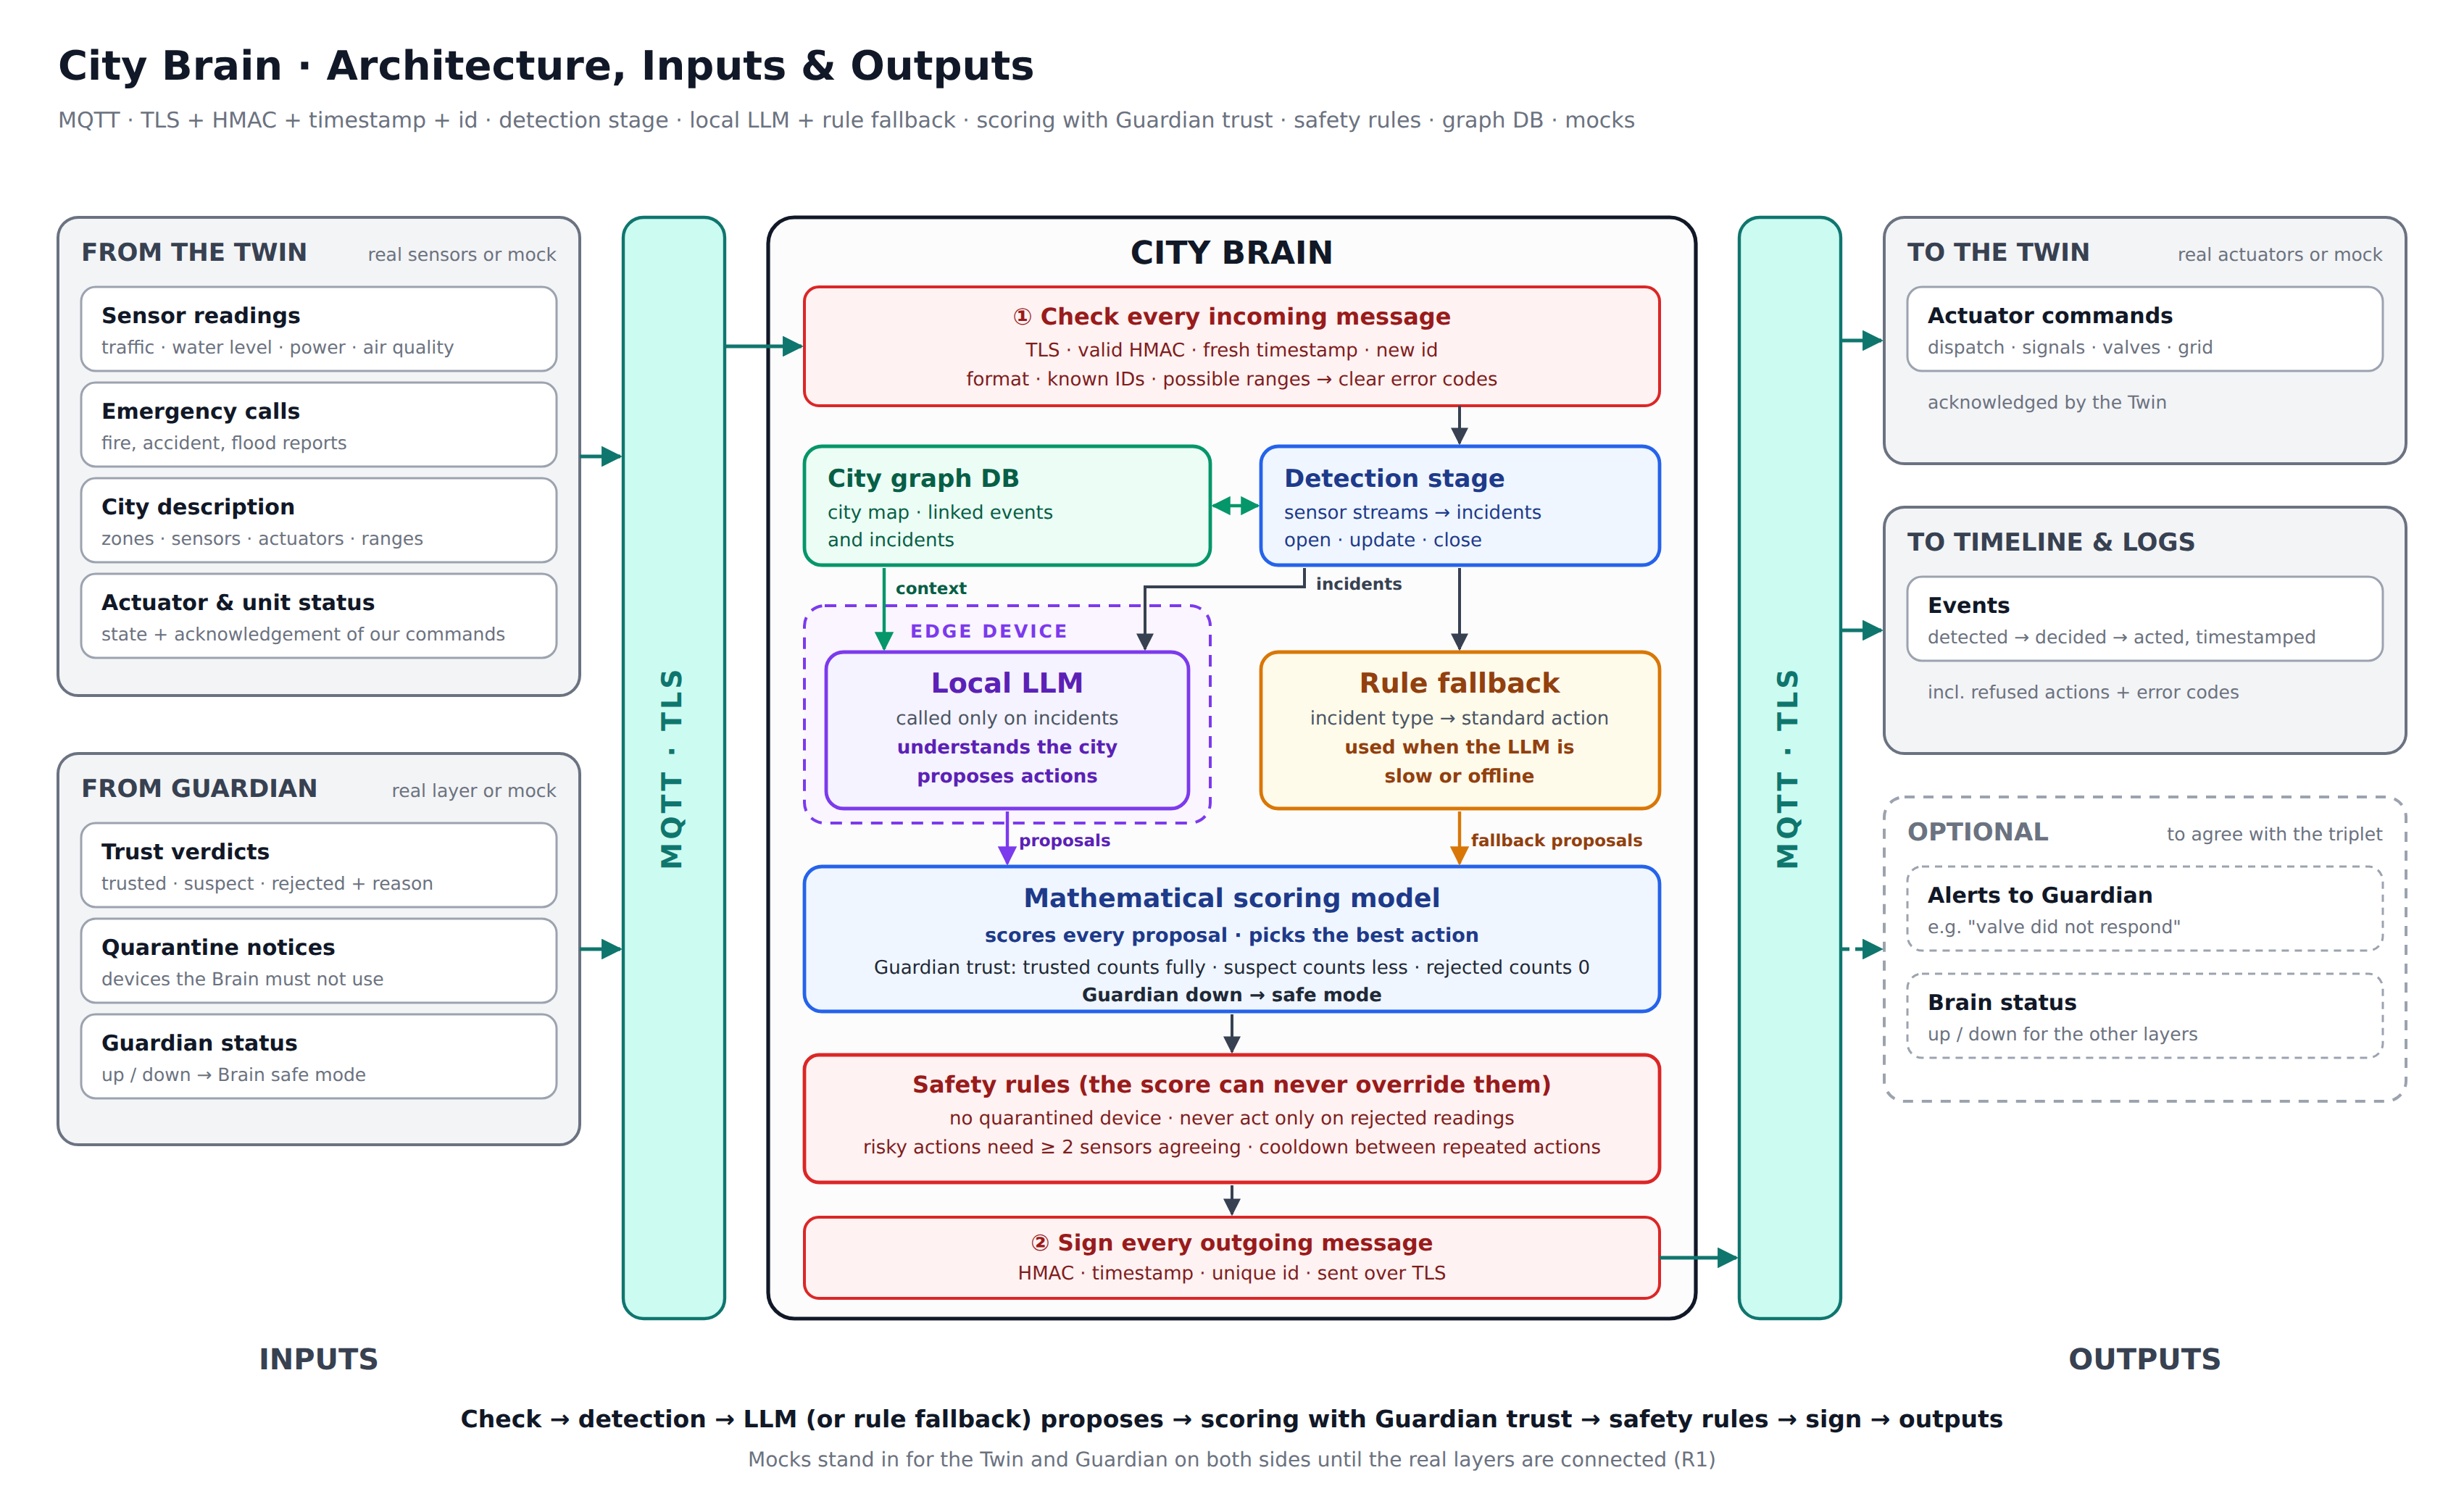
\includegraphics[width=\linewidth]{city-brain-architecture.png}
\caption{City Brain architecture: inputs from the Twin and Guardian, outputs to the Twin and the timeline. All exchanges go through the MQTT broker over TLS.}
\end{figure}

\subsection{Who sends what to whom}

\begin{tabularx}{\linewidth}{@{}l l Y@{}}
\toprule
\textbf{From} & \textbf{To} & \textbf{Content} \\
\midrule
Twin & Brain, Guardian & City description (zones, sensors, actuators, units) \\
Twin & Brain, Guardian & Sensor readings (traffic, water level, power load, air quality) \\
Twin & Brain, Guardian & Emergency calls \\
Twin & Brain & Actuator and unit state, acknowledgement of each command \\
Guardian & Brain & Trust verdicts on sensors / readings \\
Guardian & Brain, Twin & Quarantine notices for devices \\
Brain & Twin & Actuator commands (dispatch, traffic signals, valves, grid) \\
Brain & Timeline & Events (incident detected, decision, action, refusal) \\
All layers & All layers & Status: online / offline \\
\bottomrule
\end{tabularx}

\subsection{What the City Brain does with your data}
So that each team understands why each requirement exists:
\begin{enumerate}
  \item Every incoming message is \textbf{checked}: TLS, HMAC, timestamp, unique id, format, known IDs and possible range. Rejected messages are logged with an error code (Section~\ref{sec:errors}).
  \item A \textbf{detection stage} turns the sensor streams into \textbf{incidents} (flood, fire, accident, traffic jam, power problem).
  \item A local LLM and a rule-based fallback \textbf{propose actions}; a scoring model picks the best one, giving each reading a weight based on \textbf{Guardian's verdict}.
  \item \textbf{Safety rules} block any action on a quarantined device, any action based only on rejected readings, and risky actions confirmed by a single sensor.
  \item The chosen action is sent to the Twin as a \textbf{signed command}, and the Brain checks the acknowledgement.
\end{enumerate}

%-------------------------------------------------------------------
\section{Transport: MQTT}

\begin{longtable}{@{}l p{10.9cm} l@{}}
\toprule
\textbf{ID} & \textbf{Requirement} & \textbf{Level} \\
\midrule
\endhead
TR-1 & All layers exchange data only through \textbf{one shared MQTT broker} (Mosquitto proposed). & \MUST \\
TR-2 & Every client supports \textbf{MQTT 3.1.1}. MQTT 5 features are not required, so that embedded clients (e.g.\ ESP32 with real sensors) can connect. & \MUST \\
TR-3 & The broker address, port, credentials and topic prefix are read from a \textbf{configuration file}, never hard-coded. & \MUST \\
TR-4 & Each layer connects with a \textbf{fixed client id}: \code{twin}, \code{guardian}, \code{brain} (plus a suffix for extra clients, e.g.\ \code{twin-gw1}). & \SHOULD \\
TR-5 & QoS and retained flags follow the topic table in Annex~\ref{annex:topics}. & \MUST \\
TR-6 & Each layer publishes its status on \code{\{layer\}/status}: \code{online} (retained) when connected, and sets a \textbf{Last Will} \code{offline} (retained) so others are told when it disconnects. & \MUST \\
TR-7 & The broker runs on a machine connected to the \textbf{triplet's own router or hotspot}, never on the venue Wi-Fi. & \MUST \\
TR-8 & A client that loses the connection reconnects automatically and re-subscribes. & \MUST \\
\bottomrule
\end{longtable}

%-------------------------------------------------------------------
\section{Security}

\subsection{Connection security (TLS, accounts, permissions)}

\begin{longtable}{@{}l p{10.9cm} l@{}}
\toprule
\textbf{ID} & \textbf{Requirement} & \textbf{Level} \\
\midrule
\endhead
SEC-1 & The broker accepts connections only over \textbf{TLS} (port 8883). Plain port 1883 is disabled for the demo. & \MUST \\
SEC-2 & The triplet generates \textbf{one certificate authority (CA)}; every client verifies the broker certificate against it. & \MUST \\
SEC-3 & Anonymous access is disabled. Each layer has \textbf{its own username and password} (or client certificate). & \MUST \\
SEC-4 & The broker enforces the \textbf{topic permissions (ACL)} of Table~\ref{tab:acl}: each layer can publish only on its own topics. & \MUST \\
SEC-5 & Passwords, keys and certificates are kept in files excluded from Git (\code{.env}, \code{secrets/}), never in the repository. & \MUST \\
SEC-6 & Client certificates (mutual TLS) instead of passwords. & \MAY \\
\bottomrule
\end{longtable}

\begin{table}[h]
\centering
\begin{tabularx}{\linewidth}{@{}l Y Y@{}}
\toprule
\textbf{Account} & \textbf{May publish on} & \textbf{May subscribe to} \\
\midrule
\code{twin} & \code{city/\#}, \code{twin/\#} & \code{brain/cmd/\#}, \code{guardian/\allowbreak quarantine/\allowbreak \#}, \code{+/status} \\
\code{guardian} & \code{guardian/\#} & \code{city/\#}, \code{twin/\#}, \code{brain/\#}, \code{+/status} \\
\code{brain} & \code{brain/\#} & \code{city/\#}, \code{twin/\#}, \code{guardian/\#}, \code{+/status} \\
\code{timeline} & -- (read only) & \code{\#} \\
\bottomrule
\end{tabularx}
\caption{Topic permissions per account. A compromised Twin client cannot publish fake Guardian verdicts, and only the Brain can send commands.}
\label{tab:acl}
\end{table}

\subsection{Message security (HMAC, timestamp, id)}

TLS protects the connection, but inside the broker a message is readable again. The HMAC proves that each message was written by a holder of the shared secret and was not changed on the way, even through the broker.

\paragraph{Envelope.} To avoid any difference in how languages format JSON (spaces, key order, numbers), the HMAC is computed over the \textbf{exact text} of the message body. Every MQTT payload is therefore an \textbf{envelope}:

\begin{lstlisting}
{
  "v": 1,
  "body": "<the message, as a JSON text string>",
  "hmac": "<HMAC-SHA256 of the body text, lowercase hex>"
}
\end{lstlisting}

The receiver verifies the HMAC on the \code{body} text first, and only then parses the body.

\begin{longtable}{@{}l p{10.9cm} l@{}}
\toprule
\textbf{ID} & \textbf{Requirement} & \textbf{Level} \\
\midrule
\endhead
SEC-7 & Every payload uses the envelope above, with \code{"v": 1}. & \MUST \\
SEC-8 & \code{hmac} = HMAC-SHA256(key, UTF-8 bytes of \code{body}), written as 64 lowercase hexadecimal characters. & \MUST \\
SEC-9 & \textbf{One secret key per pair of layers}: Twin--Brain, Twin--Guardian, Guardian--Brain. Keys are at least 32 random bytes. & \MUST \\
SEC-10 & Messages published to several layers (readings, calls, city description, status) are signed with the key of each receiving pair, in the field \code{hmacs}: \code{\{"brain": "...", "guardian": "..."\}} instead of \code{hmac}. & \MUST \\
SEC-11 & The receiver rejects a message whose HMAC is missing or wrong (error \code{E\_AUTH}). & \MUST \\
SEC-12 & Every body has a \code{timestamp} (Section~\ref{sec:msg}). The receiver rejects a message more than \textbf{10 seconds} older or newer than its own clock (error \code{E\_STALE}). & \MUST \\
SEC-13 & Every body has a \code{id} unique for its sender. The receiver remembers the ids seen in the last 60 seconds and rejects repeats (error \code{E\_REPLAY}). & \MUST \\
SEC-14 & All machines, including sensor boards, synchronise their clocks with \textbf{NTP} from the triplet router or the broker machine, so that the 10-second window works. & \MUST \\
SEC-15 & New keys are generated before the final event if any key was shared in a chat or committed by mistake. & \SHOULD \\
\bottomrule
\end{longtable}

\paragraph{What this does not cover.} These measures stop outsiders and tampering between layers. They do not detect a sensor that sends false values with a valid HMAC, because the Twin legitimately signs its own readings. Detecting that is the Guardian layer's job (trust verdicts), and the City Brain adds its own checks (no action on rejected readings, confirmation from more than one sensor).

%-------------------------------------------------------------------
\section{Message format}
\label{sec:msg}

\subsection{Common body fields}

Every message body, in every direction, starts with these fields:

\begin{tabularx}{\linewidth}{@{}l l Y l@{}}
\toprule
\textbf{Field} & \textbf{Type} & \textbf{Meaning} & \textbf{Level} \\
\midrule
\code{id} & string & Unique message id for the sender, e.g.\ \code{twin-000182} & \MUST \\
\code{timestamp} & string & Time of sending, ISO 8601 in UTC with milliseconds, e.g.\ \code{2026-11-14T10:22:03.120Z} & \MUST \\
\code{source} & string & Sending layer: \code{twin}, \code{guardian} or \code{brain} & \MUST \\
\code{correlation\_id} & string & Id of the original message this one results from (a verdict on a reading, an acknowledgement of a command). Lets every layer and the timeline link cause and effect. & \SHOULD \\
\bottomrule
\end{tabularx}

\subsection{Naming and units}

\begin{longtable}{@{}l p{10.9cm} l@{}}
\toprule
\textbf{ID} & \textbf{Requirement} & \textbf{Level} \\
\midrule
\endhead
MSG-1 & All messages are JSON, UTF-8. Field names are \code{snake\_case}. & \MUST \\
MSG-2 & IDs use lowercase letters, digits and dashes, and are stable during a run: zones \code{port}, \code{z3}; sensors \code{water-level-04}; actuators \code{valve-port-up}; units \code{ambulance-2}. & \MUST \\
MSG-3 & Every sensor, actuator and unit id used in any message is declared in the city description (TW-1). & \MUST \\
MSG-4 & Values use the units of Table~\ref{tab:units}. & \MUST \\
MSG-5 & Unknown extra fields are ignored by the receiver, so that a layer can add information without breaking the others. & \MUST \\
MSG-6 & Message size stays under 16~KB. & \SHOULD \\
\bottomrule
\end{longtable}

\begin{table}[h]
\centering
\begin{tabularx}{0.9\linewidth}{@{}l l Y@{}}
\toprule
\textbf{Sensor type} (\code{type}) & \textbf{Unit} (\code{unit}) & \textbf{Meaning} \\
\midrule
\code{water\_level} & \code{m} & Water height above the reference level \\
\code{traffic\_speed} & \code{km/h} & Average vehicle speed \\
\code{traffic\_density} & \code{veh/km} & Vehicles per km of road \\
\code{power\_load} & \code{kW} & Electrical load \\
\code{air\_quality} & \code{ug/m3} & PM2.5 concentration \\
\code{smoke} & \code{0-1} & Smoke detector level \\
\code{temperature} & \code{degC} & Air temperature \\
\bottomrule
\end{tabularx}
\caption{Sensor types and units (the Twin team may add types; they must appear in the city description).}
\label{tab:units}
\end{table}

%-------------------------------------------------------------------
\section{Requirements on the Twin layer}

\subsection{City description}

\begin{longtable}{@{}l p{10.9cm} l@{}}
\toprule
\textbf{ID} & \textbf{Requirement} & \textbf{Level} \\
\midrule
\endhead
TW-1 & The Twin publishes the \textbf{city description} on \code{twin/meta}, \textbf{retained}, QoS 1, at start-up and whenever it changes. & \MUST \\
TW-2 & It lists every \textbf{zone} with its neighbours (\code{adjacent}), every \textbf{sensor} with type, zone, unit, possible range (\code{min}, \code{max}) and alert level, every \textbf{actuator} with the zones it controls and the actions it accepts, and every \textbf{unit} (ambulance, fire, police, rescue). & \MUST \\
TW-3 & Zone \code{type} and \code{exposure} (e.g.\ hospital, school) are included. & \SHOULD \\
\bottomrule
\end{longtable}

\begin{lstlisting}[caption={Body of the city description (shortened)}]
{
  "id": "twin-meta-001", "timestamp": "2026-11-14T09:00:00.000Z", "source": "twin",
  "zones": [
    {"zone_id": "port", "name": "Port", "type": "port", "exposure": "high",
     "adjacent": ["docks", "z4"]}
  ],
  "sensors": [
    {"sensor_id": "water-level-04", "zone_id": "port", "type": "water_level",
     "unit": "m", "min": 0.0, "max": 4.0, "alert": 2.0}
  ],
  "actuators": [
    {"actuator_id": "valve-port-up", "type": "valve", "zone_id": "port",
     "controls": ["port", "docks"], "actions": ["open", "close"]}
  ],
  "units": [
    {"unit_id": "ambulance-2", "type": "ambulance", "home_zone": "z3"}
  ]
}
\end{lstlisting}

\subsection{Sensor readings}

\begin{longtable}{@{}l p{10.9cm} l@{}}
\toprule
\textbf{ID} & \textbf{Requirement} & \textbf{Level} \\
\midrule
\endhead
TW-4 & Readings are published on \code{city/\allowbreak \{zone\_id\}/\allowbreak sensor/\allowbreak \{type\}/\allowbreak \{sensor\_id\}}, QoS 0. & \MUST \\
TW-5 & The body contains \code{sensor\_id}, \code{zone\_id}, \code{type}, \code{value} (number) and \code{unit}. & \MUST \\
TW-6 & Each sensor publishes at least \textbf{every 5 seconds}. & \MUST \\
TW-7 & Each sensor publishes every second. & \SHOULD \\
TW-8 & Real sensors are published through a gateway or board that applies the same envelope, HMAC, timestamp and id rules. & \MUST \\
\bottomrule
\end{longtable}

\begin{lstlisting}[caption={Body of a sensor reading}]
{"id": "twin-000182", "timestamp": "2026-11-14T10:22:03.120Z", "source": "twin",
 "sensor_id": "water-level-04", "zone_id": "port",
 "type": "water_level", "value": 2.4, "unit": "m"}
\end{lstlisting}

\subsection{Emergency calls}

\begin{longtable}{@{}l p{10.9cm} l@{}}
\toprule
\textbf{ID} & \textbf{Requirement} & \textbf{Level} \\
\midrule
\endhead
TW-9 & Calls are published on \code{city/\allowbreak \{zone\_id\}/\allowbreak call}, QoS 1, with \code{call\_id}, \code{zone\_id} and \code{category} (\code{fire}, \code{accident}, \code{flood}, \code{medical}, \code{other}). & \MUST \\
TW-10 & Calls include a short free-text description in \code{text} (max.\ 280 characters). & \SHOULD \\
\bottomrule
\end{longtable}

\begin{lstlisting}[caption={Body of an emergency call}]
{"id": "twin-000190", "timestamp": "2026-11-14T10:22:05.004Z", "source": "twin",
 "call_id": "call-0012", "zone_id": "z3", "category": "fire",
 "text": "Smoke coming from the substation"}
\end{lstlisting}

\subsection{Commands and acknowledgements}

\begin{longtable}{@{}l p{10.9cm} l@{}}
\toprule
\textbf{ID} & \textbf{Requirement} & \textbf{Level} \\
\midrule
\endhead
TW-11 & The Twin subscribes to \code{brain/cmd/\#} and executes valid commands (format in BR-1). & \MUST \\
TW-12 & A command with an \code{id} already executed is \textbf{not executed again} (MQTT QoS 1 can deliver a message twice). & \MUST \\
TW-13 & For every command, the Twin publishes an \textbf{acknowledgement} on \code{twin/\allowbreak actuator/\allowbreak \{actuator\_id\}} (or \code{twin/\allowbreak unit/\allowbreak \{unit\_id\}}) within \textbf{2 seconds}, QoS 1, with \code{correlation\_id} = the command \code{id}, \code{result} (\code{done}, \code{rejected}, \code{failed}), the new \code{state} and, if not done, a \code{reason}. & \MUST \\
TW-14 & The Twin also publishes the actuator state on the same topic whenever it changes, retained. & \SHOULD \\
TW-15 & Unit status (\code{free}, \code{en\_route}, \code{on\_scene}, \code{returning}) and current zone are published on \code{twin/\allowbreak unit/\allowbreak \{unit\_id\}}, retained, whenever they change. & \MUST \\
TW-16 & Actions have a \textbf{visible effect on later readings} (valve opened $\rightarrow$ water level stops rising; signals retimed $\rightarrow$ traffic speed rises), so that the Brain can check its action worked. & \SHOULD \\
TW-17 & The Twin refuses commands to a device quarantined by Guardian, with \code{result: rejected}, \code{reason: quarantined}. & \SHOULD \\
\bottomrule
\end{longtable}

\begin{lstlisting}[caption={Body of an acknowledgement}]
{"id": "twin-000205", "timestamp": "2026-11-14T10:22:04.410Z", "source": "twin",
 "correlation_id": "brain-000042",
 "actuator_id": "valve-port-up", "result": "done", "state": "open_80"}
\end{lstlisting}

\subsection{Scenarios and status}

\begin{longtable}{@{}l p{10.9cm} l@{}}
\toprule
\textbf{ID} & \textbf{Requirement} & \textbf{Level} \\
\midrule
\endhead
TW-18 & The Twin publishes \code{twin/status} with Last Will (TR-6). & \MUST \\
TW-19 & The Twin can play each Test Book scenario from one command, including \textbf{faulty or fake readings} (stuck value, spike, false flood), which are still correctly signed. & \SHOULD \\
\bottomrule
\end{longtable}

%-------------------------------------------------------------------
\section{Requirements on the Guardian layer}

\subsection{Trust verdicts}

\begin{longtable}{@{}l p{10.9cm} l@{}}
\toprule
\textbf{ID} & \textbf{Requirement} & \textbf{Level} \\
\midrule
\endhead
GD-1 & Guardian publishes a verdict per sensor on \code{guardian/\allowbreak verdict/\allowbreak \{sensor\_id\}}, \textbf{retained}, QoS 1. & \MUST \\
GD-2 & The body contains \code{sensor\_id}, \code{verdict} (\code{trusted}, \code{suspect}, \code{rejected}) and \code{reason} (code from Table~\ref{tab:reasons}). & \MUST \\
GD-3 & When the verdict is about a specific reading, \code{correlation\_id} is that reading's \code{id}. & \SHOULD \\
GD-4 & A new verdict is published \textbf{as soon as it changes}, and at most \textbf{10 seconds} after a faulty or fake reading appears. & \MUST \\
GD-5 & The current verdict of every sensor is re-published at least every 10 seconds, so the Brain knows it is still valid. & \SHOULD \\
GD-6 & A sensor that Guardian isolates is published with \code{verdict: rejected}, \code{reason: isolated}. & \MUST \\
\bottomrule
\end{longtable}

\begin{table}[h]
\centering
\begin{tabularx}{0.9\linewidth}{@{}l Y@{}}
\toprule
\textbf{Reason code} & \textbf{Meaning} \\
\midrule
\code{ok} & Nothing wrong found \\
\code{out\_of\_range} & Value outside the possible range \\
\code{stuck\_value} & Value not changing when it should \\
\code{spike} & Sudden jump not explained by neighbours \\
\code{drift} & Slow deviation from the sensor's normal behaviour \\
\code{inconsistent} & Contradicts neighbouring sensors \\
\code{replay} & Old message sent again \\
\code{bad\_signature} & HMAC missing or wrong \\
\code{flooding} & Device sends far too many messages \\
\code{isolated} & Sensor isolated by Guardian \\
\code{other} & Any other reason (details in \code{details}) \\
\bottomrule
\end{tabularx}
\caption{Proposed verdict reason codes.}
\label{tab:reasons}
\end{table}

\begin{lstlisting}[caption={Body of a verdict}]
{"id": "guardian-004521", "timestamp": "2026-11-14T10:22:03.900Z", "source": "guardian",
 "correlation_id": "twin-000182",
 "sensor_id": "water-level-04", "verdict": "rejected", "reason": "out_of_range"}
\end{lstlisting}

\subsection{Quarantine and status}

\begin{longtable}{@{}l p{10.9cm} l@{}}
\toprule
\textbf{ID} & \textbf{Requirement} & \textbf{Level} \\
\midrule
\endhead
GD-7 & Quarantine notices are published on \code{guardian/\allowbreak quarantine/\allowbreak \{device\_id\}}, \textbf{retained}, QoS 1, with \code{device\_id}, \code{state} (\code{quarantined} or \code{released}) and \code{reason}. & \MUST \\
GD-8 & Guardian publishes \code{guardian/status} with Last Will (TR-6). When Guardian is offline, the Brain switches to safe mode. & \MUST \\
GD-9 & Guardian subscribes to \code{brain/alert} to receive the Brain's alerts (e.g.\ an actuator that does not respond). & \MAY \\
\bottomrule
\end{longtable}

\begin{lstlisting}[caption={Body of a quarantine notice}]
{"id": "guardian-004530", "timestamp": "2026-11-14T10:23:10.000Z", "source": "guardian",
 "device_id": "valve-port-main", "state": "quarantined", "reason": "inconsistent"}
\end{lstlisting}

%-------------------------------------------------------------------
\section{What the City Brain layer provides}

These are our commitments, so that the other teams can build their mocks of the Brain.

\begin{longtable}{@{}l p{10.9cm} l@{}}
\toprule
\textbf{ID} & \textbf{Commitment} & \textbf{Level} \\
\midrule
\endhead
BR-1 & Commands are published on \code{brain/\allowbreak cmd/\allowbreak \{actuator\_id\}} or \code{brain/\allowbreak cmd/\allowbreak \{unit\_id\}}, QoS 1, with \code{actuator\_id} or \code{unit\_id}, \code{action} (one of the actions declared in the city description, or \code{dispatch} for units), \code{params}, \code{incident\_id} and a short \code{reason}. & \MUST \\
BR-2 & The Brain never sends a command to a quarantined device and never acts only on rejected readings. & \MUST \\
BR-3 & The Brain publishes its events for the timeline on \code{brain/event}: incident opened / updated / closed, decision, command sent, acknowledgement received, action refused. & \MUST \\
BR-4 & The Brain publishes \code{brain/status} with Last Will (TR-6). & \MUST \\
BR-5 & Every message the Brain rejects is reported on \code{brain/error} with the error code, the topic and the message \code{id}, so partners can debug quickly. & \SHOULD \\
BR-6 & The Brain publishes alerts on \code{brain/alert} (e.g.\ \code{actuator\_not\_responding}). & \MAY \\
\bottomrule
\end{longtable}

\begin{lstlisting}[caption={Body of a command}]
{"id": "brain-000042", "timestamp": "2026-11-14T10:22:04.020Z", "source": "brain",
 "correlation_id": "twin-000182",
 "actuator_id": "valve-port-up", "action": "open", "params": {"percent": 80},
 "incident_id": "inc-0031", "reason": "flood at port"}
\end{lstlisting}

\begin{lstlisting}[caption={Body of a unit dispatch}]
{"id": "brain-000043", "timestamp": "2026-11-14T10:22:06.500Z", "source": "brain",
 "correlation_id": "twin-000190",
 "unit_id": "fire-1", "action": "dispatch", "params": {"zone_id": "z3"},
 "incident_id": "inc-0032", "reason": "fire in zone z3"}
\end{lstlisting}

\begin{lstlisting}[caption={Body of a timeline event}]
{"id": "brain-000044", "timestamp": "2026-11-14T10:22:04.025Z", "source": "brain",
 "correlation_id": "twin-000182",
 "event": "command_sent", "incident_id": "inc-0031",
 "summary": "flood at port -> open valve-port-up 80%"}
\end{lstlisting}

%-------------------------------------------------------------------
\section{Error handling}
\label{sec:errors}

Every layer applies the same checks to what it receives, and uses the same error codes in its logs:

\begin{tabularx}{\linewidth}{@{}l Y Y@{}}
\toprule
\textbf{Code} & \textbf{Rejected when} & \textbf{Example} \\
\midrule
\code{E\_FORMAT} & Envelope or body is not valid JSON, or a required field is missing or has the wrong type & Reading without \code{value} \\
\code{E\_AUTH} & HMAC missing or wrong & Message changed in transit \\
\code{E\_STALE} & Timestamp more than 10 s away from the receiver's clock & Old message, or clock not synchronised \\
\code{E\_REPLAY} & \code{id} already received in the last 60 s & Captured message sent again \\
\code{E\_UNKNOWN\_ID} & Sensor, zone, actuator or unit not in the city description & \code{valve-x9} does not exist \\
\code{E\_RANGE} & Value outside the declared \code{min}/\code{max} & Water level $-5$ m \\
\bottomrule
\end{tabularx}

\medskip
A rejected message is \textbf{never processed further}. It is logged with its code, and shown on the timeline.

%-------------------------------------------------------------------
\section{Mocks and integration tests}

\subsection{Shared examples and mocks}
\begin{itemize}
  \item The example messages of this book are stored in the triplet repository as JSON files (\code{docs/\allowbreak interface/\allowbreak examples/\allowbreak }). Every team builds its mocks from these files, so that mocks and real layers match.
  \item Each team runs its layer alone with mocks of the other two (R1), using the same broker configuration, topics, envelope and HMAC.
  \item The HMAC test vector of Annex~\ref{annex:hmac} is checked by every team's code before the first joint run.
\end{itemize}

\subsection{Interface tests}

These tests check the interfaces only. They come before the functional Test Book scenarios.

\begin{longtable}{@{}l p{8.4cm} p{4.6cm}@{}}
\toprule
\textbf{ID} & \textbf{Test} & \textbf{Expected result} \\
\midrule
\endhead
IT-1 & Brain starts after the Twin & Brain receives the retained city description \\
IT-2 & Twin publishes a valid reading & Accepted by Brain and Guardian \\
IT-3 & A reading with a wrong HMAC & Rejected, \code{E\_AUTH} \\
IT-4 & A reading 30 s old & Rejected, \code{E\_STALE} \\
IT-5 & The same reading sent twice & Second one rejected, \code{E\_REPLAY} \\
IT-6 & A reading from an undeclared sensor & Rejected, \code{E\_UNKNOWN\_ID} \\
IT-7 & Guardian rejects a fake flood reading & Brain sends no command, logs the reason \\
IT-8 & Guardian quarantines a valve & Brain uses another valve or none \\
IT-9 & Brain sends a command & Twin acknowledges within 2 s; a duplicate is not executed \\
IT-10 & Guardian is stopped & \code{guardian/\allowbreak status = offline}; Brain switches to safe mode \\
IT-11 & Twin is stopped & \code{twin/\allowbreak status = offline}; Brain and Guardian log it \\
IT-12 & A client without credentials, or publishing on another layer's topic & Refused by the broker \\
\bottomrule
\end{longtable}

%-------------------------------------------------------------------
\section{Open points to agree}

\begin{tabularx}{\linewidth}{@{}l Y l@{}}
\toprule
\textbf{\#} & \textbf{Point} & \textbf{With} \\
\midrule
1 & Final topic names and the envelope format (Section 4.2) & All \\
2 & Which machine hosts the broker; who creates the CA, certificates and accounts & All \\
3 & How the three HMAC keys are generated and shared & All \\
4 & Timestamp window (10 s) and id memory (60 s) & All \\
5 & Sensor types, units and reading frequency of the real sensors & Twin \\
6 & Actions accepted by each actuator type; unit types & Twin \\
7 & Whether emergency calls include free text & Twin \\
8 & Verdict per sensor or per reading; reason codes & Guardian \\
9 & Whether \code{brain/alert} is used & Guardian \\
10 & Who builds the shared timeline screen (it subscribes to all topics) & All \\
11 & Interface freeze date and first joint run date & All \\
\bottomrule
\end{tabularx}

%-------------------------------------------------------------------
\appendix
\section{Topic summary}
\label{annex:topics}

{\small\begin{longtable}{@{}p{6.3cm} l p{2.6cm} c c@{}}
\toprule
\textbf{Topic} & \textbf{Publisher} & \textbf{Subscribers} & \textbf{QoS} & \textbf{Retained} \\
\midrule
\endhead
\code{twin/meta} & Twin & Brain, Guardian & 1 & yes \\
\code{city/\allowbreak \{zone\}/\allowbreak sensor/\allowbreak \{type\}/\allowbreak \{sensor\}} & Twin & Brain, Guardian & 0 & no \\
\code{city/\{zone\}/call} & Twin & Brain, Guardian & 1 & no \\
\code{twin/\allowbreak actuator/\allowbreak \{actuator\}} & Twin & Brain, Guardian & 1 & state: yes \\
\code{twin/unit/\{unit\}} & Twin & Brain & 1 & yes \\
\code{guardian/\allowbreak verdict/\allowbreak \{sensor\}} & Guardian & Brain & 1 & yes \\
\code{guardian/\allowbreak quarantine/\allowbreak \{device\}} & Guardian & Brain, Twin & 1 & yes \\
\code{brain/\allowbreak cmd/\allowbreak \{actuator or unit\}} & Brain & Twin & 1 & no \\
\code{brain/event} & Brain & Timeline & 0 & no \\
\code{brain/error} & Brain & All & 0 & no \\
\code{brain/alert} & Brain & Guardian & 1 & no \\
\code{\{twin,guardian,brain\}/\allowbreak status} & each layer & all & 1 & yes \\
\bottomrule
\end{longtable}}

\section{HMAC reference implementation and test vector}
\label{annex:hmac}

\subsection{Python}
\begin{lstlisting}[language=Python]
import hmac, hashlib, json

def seal(body: dict, key: bytes) -> str:
    text = json.dumps(body, separators=(",", ":"))
    tag = hmac.new(key, text.encode("utf-8"), hashlib.sha256).hexdigest()
    return json.dumps({"v": 1, "body": text, "hmac": tag})

def open_sealed(payload: str, key: bytes) -> dict:
    env = json.loads(payload)
    text = env["body"]
    expected = hmac.new(key, text.encode("utf-8"), hashlib.sha256).hexdigest()
    if not hmac.compare_digest(expected, env.get("hmac", "")):
        raise ValueError("E_AUTH")
    return json.loads(text)          # then check timestamp, id, format, ids, range
\end{lstlisting}

\subsection{Test vector}
Every implementation must give exactly this result.

\begin{tabularx}{\linewidth}{@{}l Y@{}}
\toprule
Key (UTF-8 text) & \code{test-secret-twin-brain} \\
Body text & see below \\
Expected HMAC & \code{c97ecfbc4f3f1c82140c3bd78d804b33}\linebreak\code{11af0bf051d5c98f025aef9f76b6771b} \\
\bottomrule
\end{tabularx}

\begin{lstlisting}
{"correlation_id":"twin-000182","id":"twin-000182","sensor_id":"water-level-04","source":"twin","timestamp":"2026-11-14T10:22:03.120Z","type":"water_level","unit":"m","value":2.4,"zone_id":"port"}
\end{lstlisting}

\textit{The key above is for testing only. Never use it in the real system.}

\end{document}
